\documentclass[rgb]{beamer}

\usepackage[english]{babel}
\usepackage[utf8]{inputenc}
\usepackage{xcolor}
\usepackage{listings}
\usepackage{adjustbox}
\usepackage{amsmath}
\usepackage{multirow}
\usepackage[linewidth=1pt]{mdframed}

% Graphics
\usepackage{graphicx}

\usepackage{tikz}
\usetikzlibrary{calc,shapes.multipart,chains,arrows}

% Font
\usepackage{paratype}
\setbeamerfont{frametitle}{family=\bf}

% Beamer theme settings
\usecolortheme{seagull}
\setbeamertemplate{itemize item}{\raisebox{0.8mm}{\rule{1.8mm}{1.2mm}}}
\usenavigationsymbolstemplate{} % no navigation buttons

\usepackage{listings}

% Define Language
\lstdefinelanguage{fsharp}
{
  % list of keywords
  morekeywords={
    and,
    do,
    else,
    exception,
    for,
    fun,
    function,
    if,
    in,
    let,
    match,
    module,
    mutable,
    open,
    of,
    rec,
    then,
    try,
    type,
    unsafe,
    use,
    val,
    when,
    while,
    with,
  },
  sensitive=true, % keywords are not case-sensitive
  morecomment=[l]{//}, % l is for line comment
%  otherkeywords={>,<,=,<=,>=,!,*,/,-,+,|,&,||,&&,==,=>},
  morestring=[b]" % defines that strings are enclosed in double quotes
}

% Define Colors
\usepackage{color}
\definecolor{eclipseBlue}{RGB}{42,0.0,255}
\definecolor{eclipseGreen}{RGB}{63,127,95}
\definecolor{eclipsePurple}{RGB}{127,0,85}

\newcommand{\fop}[1]{\mbox{\ttfamily\color{eclipseBlue}#1}}
\newcommand{\fw}[1]{\mbox{\ttfamily\bfseries\color{eclipsePurple}#1}}

% Set Language
\lstset{
  language={fsharp},
  basicstyle=\ttfamily, % Global Code Style
  captionpos=b, % Position of the Caption (t for top, b for bottom)
  extendedchars=true, % Allows 256 instead of 128 ASCII characters
  tabsize=2, % number of spaces indented when discovering a tab
  columns=fixed, % make all characters equal width
  keepspaces=true, % does not ignore spaces to fit width, convert tabs to spaces
  showstringspaces=false, % lets spaces in strings appear as real spaces
  breaklines=true, % wrap lines if they don't fit
  frame=trbl, % draw a frame at the top, right, left and bottom of the listing
  frameround=tttt, % make the frame round at all four corners
  framesep=4pt, % quarter circle size of the round corners
  numbers=left, % show line numbers at the left
  numberstyle=\small\ttfamily, % style of the line numbers
  commentstyle=\slshape\bfseries\color{eclipseGreen}, % style of comments
  keywordstyle=\bfseries\color{eclipsePurple}, % style of keywords
  stringstyle=\color{eclipseBlue}, % style of strings
  emph=[1] {
    false,
    true,
    Set,
    Map,
    List,
    ImgUtil,
    Pegs,
    String,
    Array,
    Array2D
  },
  emphstyle=[1]{\color{eclipseBlue}},
  moredelim=**[is][\color{red}]{@@}{@@}
}

\newcommand{\theyear}{2020}
\newcommand{\sem}[1]{[\![#1]\!]}
\newcommand{\seme}[1]{\sem{#1}\varepsilon}
\newcommand{\semzero}[1]{\sem{#1}_0}

\newcommand{\emptymap}{\{\}}
\newcommand{\fracc}[2]{\begin{eqnarray} \frac{\begin{array}{c} #1
    \end{array}}{\begin{array}{c} #2 \end{array}} \end{eqnarray}}
\newcommand{\sembox}[1]{\hfill \normalfont \mbox{\fbox{\(#1\)}}}
\newcommand{\sempart}[2]{\subsubsection*{\rm\em #1 \sembox{#2}}}
\newcommand{\axiom}[1]{\begin{eqnarray} \begin{array}{c} #1 \end{array} \end{eqnarray}}
\newcommand{\fraccn}[2]{\refstepcounter{equation}\mbox{$\frac{\begin{array}{c} #1 \end{array}}{\begin{array}{c} #2 \end{array}}$}~(\arabic{equation})}
\newcommand{\fraccc}[2]{\mbox{$\frac{\begin{array}{c} #1 \end{array}}{\begin{array}{c} #2 \end{array}}$}}
\newcommand{\onepart}[1]{\noindent\hfill#1\hfill~\vspace{2mm}}
\newcommand{\twopart}[2]{\noindent\hfill#1\hfill#2\hfill~\vspace{2mm}}
\newcommand{\threepart}[3]{\noindent\hfill#1\hfill#2\hfill#3\hfill~\vspace{2mm}}
%\newcommand{\axiomm}[1]{\refstepcounter{equation}\mbox{$\begin{array}{c} #1 \end{array}$}~(\arabic{equation})}
\newcommand{\axiomm}[1]{$\begin{array}{c} #1 \end{array}$}
%\newcommand{\ar}[1]{\stackrel{#1}{\longrightarrow}}
\newcommand{\vd}{\vdash}
\newcommand{\Ran}{{\rm Ran}}
\newcommand{\Dom}{{\rm Dom}}
\newcommand{\kw}[1]{\texttt{#1}}
\newcommand{\id}[1]{\mbox{\it{#1}}}
\newcommand{\rarr}{\rightarrow}
\newcommand{\eval}{\rarr}
\newcommand{\evals}{\leadsto}
\newcommand{\larr}{\leftarrow}

\newcommand{\head}[1]{\vspace{3mm} \textbf{\normalsize #1}}
\newcommand{\headsp}[1]{\head{#1}\vspace{1ex}}
\newcommand{\size}{\ensuremath{\mathrm{size}}}
\renewcommand{\log}{\ensuremath{\mathrm{log}}}

\newcommand{\setallthemecolors}[1]{%
\setbeamercolor*{palette primary}{use=structure,fg=white,bg=#1}%
\setbeamercolor*{palette secondary}{use=structure,fg=white,bg=#1}%
\setbeamercolor*{palette tertiary}{use=structure,fg=white,bg=#1}}

\definecolor{black}{RGB}{0,0,0}
\definecolor{maroon}{RGB}{128,0,0}
\definecolor{olive}{RGB}{128,128,0}
\definecolor{green}{RGB}{0,128,0}
\definecolor{purple}{RGB}{128,0,128}
\definecolor{teal}{RGB}{0,128,128}
\definecolor{darkteal}{RGB}{0,92,92}
\definecolor{navy}{RGB}{0,0,128}
\definecolor{gray}{RGB}{128,128,128}
\definecolor{darkgray}{RGB}{60,60,60}
\definecolor{darkred}{RGB}{139,0,0}

%palette

% #173F5F (dark blue)
\definecolor{darkblue}{RGB}{23,63,95}
% #20639B (blue)
\definecolor{blue}{RGB}{32,99,155}
% #3CAEA3 (green)
\definecolor{magenta}{RGB}{60,174,163}
% #F6D55C (yellow)
\definecolor{yellow}{RGB}{246,213,92}
% #ED553B (red)
\definecolor{red}{RGB}{237,85,59}


\usecolortheme{whale}
\useoutertheme{infolines}
\useinnertheme{rectangles}

\newcommand{\popsettitle}[2]{%
\setallthemecolors{#1}%
\newcommand{\popemne}{#2}%
\title{Programmering og Problemløsning}%
\subtitle{#2}%
\author{Martin Elsman}%
\date{}%
\institute[DIKU]{Datalogisk Institut, Københavns Universitet (DIKU)}}

\newcommand{\popmaketitleframe}{%
  \frame{\titlepage%
   \vspace{-15mm}%
   \par\noindent\rule{\textwidth}{0.4pt}%

   \vspace{4mm}%
   \tableofcontents%
   \vspace{-4mm}%
   \par\noindent\rule{\textwidth}{0.4pt}%
  }%
  \section*{\popemne}%
}


\popsettitle{blue}{Rekursion (Del 3)}  % see ../util.tex for colors

\begin{document}

\popmaketitleframe

%%%%%%%%%%%%%%%%%%%%%%%%%%%%%%%%%%%%%%%%%%%%%%%%
\subsection{Rekursion og sortering}
%%%%%%%%%%%%%%%%%%%%%%%%%%%%%%%%%%%%%%%%%%%%%%%%

\begin{frame}[fragile]
\begin{footnotesize}

  \head{Rekursion}

  \begin{quote}
    En metode for hvilken en løsning til et problem findes ved at løse
    \emph{mindre instanser} af det samme problem.
  \end{quote}

  \begin{itemize}
  \item Rekursion kan anvendes til at løse en lang række forskellige problemstillinger.

  \item I dag vil vi se på brug af rekursion i forbindelse med sortering.
  \end{itemize}

  \begin{minipage}[b]{0.6\textwidth}
  \head{Sorteringsalgoritmer}
  \begin{itemize}
  \item Insertion sort
  \item Bubble sort
  \item Selection sort
  \item Mergesort
  \item Quicksort
%  \item Quicksort (in-place array)
  \end{itemize}
\end{minipage}  \begin{minipage}[b]{0.3\textwidth}

  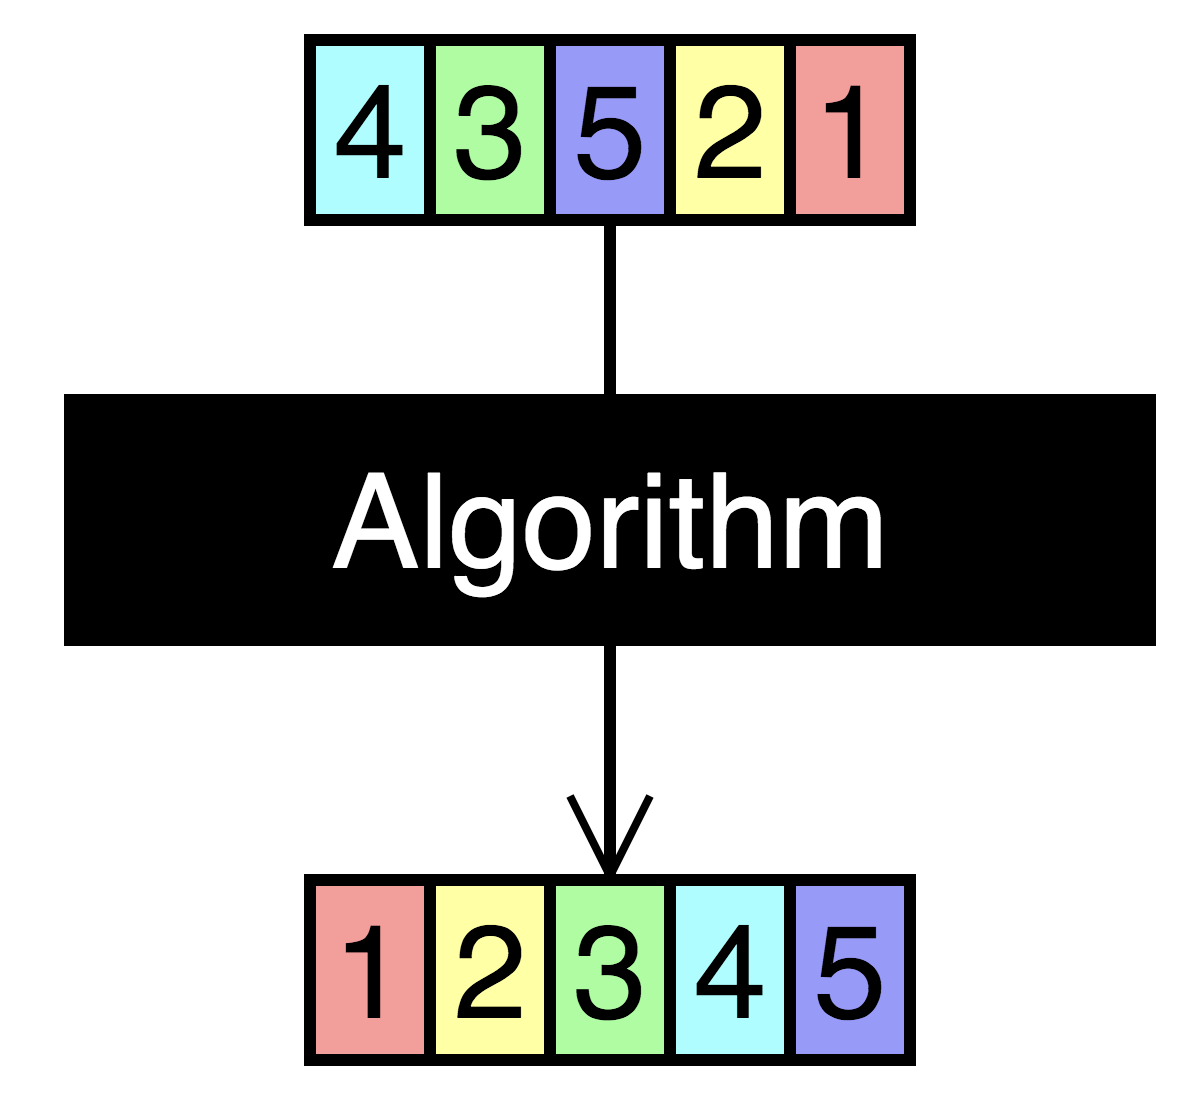
\includegraphics[width=\textwidth]{../images/sorting_algorithms.png}
\end{minipage}
\end{footnotesize}
\end{frame}

\subsection{Insertion sort}
\begin{frame}[fragile]
\begin{footnotesize}

  \head{Insertion sort}

  \begin{itemize}
  \item Gennemløb en liste et element af gangen.
  \item For hvert element, indsæt det på rette plads i resultatlisten.
  \end{itemize}

  \head{En implementation i F\#:}

\begin{lstlisting}[numbers=none,frame=none,mathescape]
let rec insert xs y =
  match xs with
    | [] -> [y]
    | x::xs' -> if y < x then y :: xs
                else x :: insert xs' y

let isort xs = List.fold (fun acc x -> insert acc x) [] xs

let xs = [7;55;34;23;5;42;32;34;8]
do printf "%A\n" (isort xs)
\end{lstlisting}

\head{Bemærk:}
\begin{itemize}
\item Nøgleordet \lstinline{rec} er nødvendigt før en funktion kan henvise til sig selv...
\item \lstinline{List.fold} benyttes til gennemløb og opbygning af ny sorteret liste.
\end{itemize}
\end{footnotesize}
\end{frame}

\begin{frame}[fragile]
\begin{footnotesize}
\head{Analyse af insertion sort}

\vspace{1ex}

\begin{minipage}[b]{0.55\textwidth}

  Funktionen \lstinline{insert} køres $N$ gange og for hver kørsel
  gennemløbes (i gennemsnit) en fjerdedel af listen ($N/4$ elementer).

\vspace{1ex}

\head{Summary:}

\vspace{1ex}
  \begin{tabular}{ll}
    Best time: & $O(N)$ \\
    Worst time: & $O(N^2)$ \\
    Average time: & $O(N^2)$
  \end{tabular}

  \vspace{1ex}
  I bedste tilfælde er listen omvendt sorteret hvorved \lstinline{insert} altid kører i konstant tid...

  \vspace{1ex}
  I animationen insættes elementerne bagfra...
  \vfill
\mbox{ }
\end{minipage} \hspace{1cm}
\begin{minipage}[b]{0.3\textwidth}

  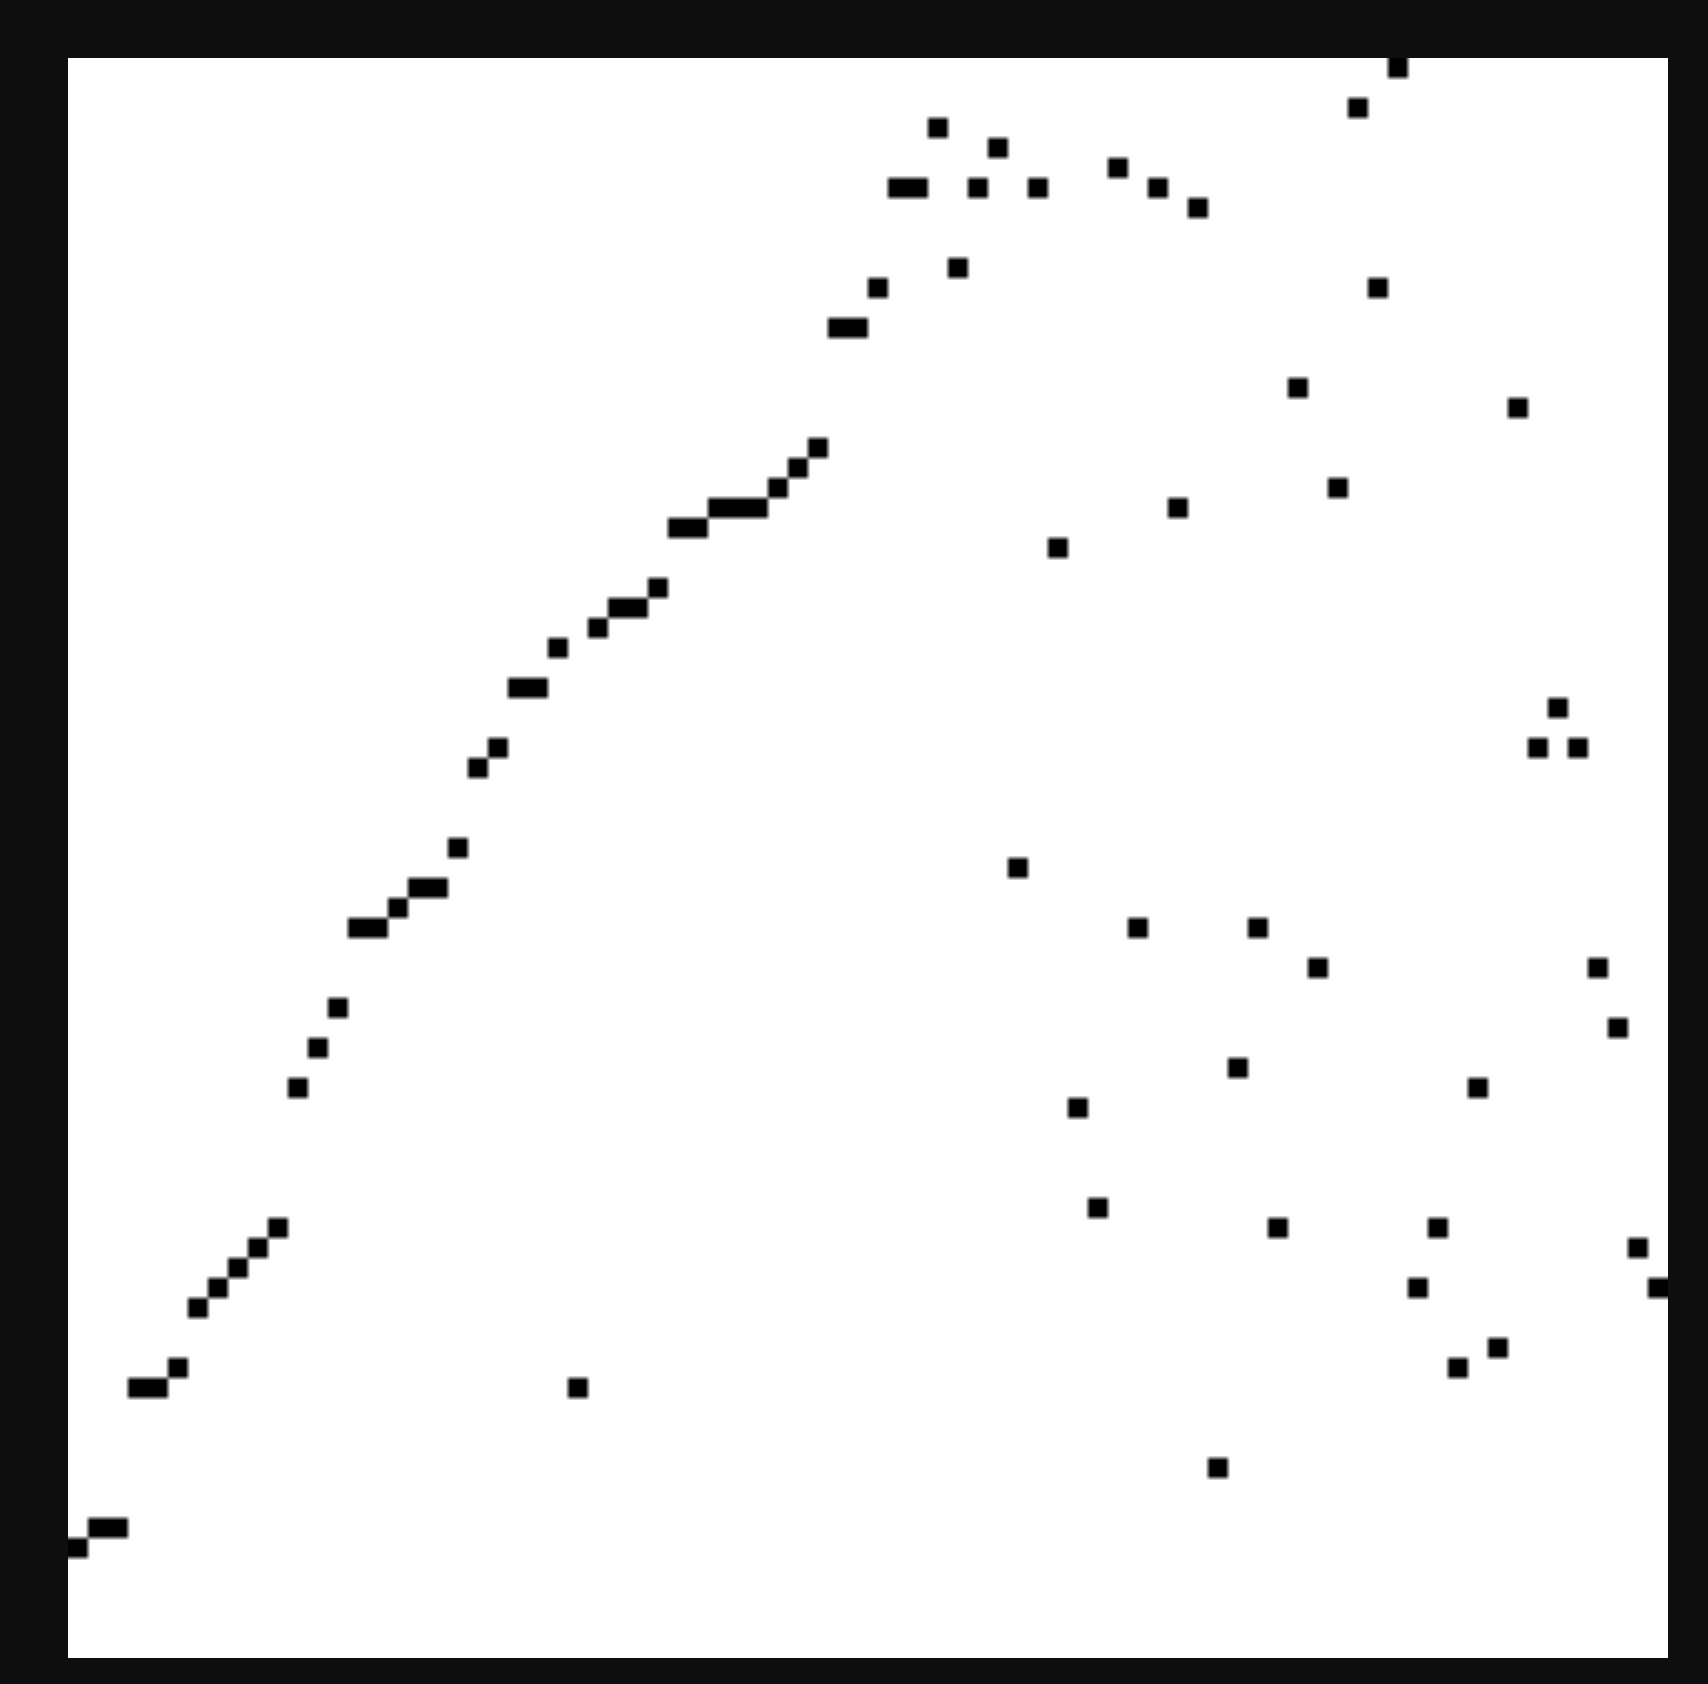
\includegraphics[width=\textwidth]{../images/isort_gif.png}

  (\href{https://upload.wikimedia.org/wikipedia/commons/a/ad/Insertion_Sort_Animation.gif}{animation})
\end{minipage}

\head{Kørsel:}

\begin{verbatim}
bash-3.2$ fsharpc --nologo isort.fs && mono isort.exe
[5; 7; 8; 23; 32; 34; 34; 42; 55]
\end{verbatim}

\end{footnotesize}
\end{frame}

\subsection{Bubble sort}
\begin{frame}[fragile]
\begin{footnotesize}

  \head{Bubble sort}

  \begin{itemize}
  \item Listen \lstinline{xs} gennemløbes $N =$ \lstinline{List.length xs} gange.
  \item For hvert gennemløb, ombyt sidestillede elementer der er forkert ordnet (bubble).
  \end{itemize}

  \head{En implementation i F\#:}

\begin{lstlisting}[numbers=none,frame=none,mathescape]
let rec bubble (xs:int list) =
  match xs with
    | x::y::ys -> if y<x then y::bubble (x::ys)
                  else x::bubble (y::ys)
    | _ -> xs

let bsort xs =
  List.fold (fun acc _ -> bubble acc) xs xs
\end{lstlisting}

\head{Bemærk:}
\begin{itemize}
\item \lstinline{List.fold} benyttes til at foretage $N$ kald af \lstinline{bubble}.
\end{itemize}
\end{footnotesize}
\end{frame}

\begin{frame}[fragile]
\begin{footnotesize}

\head{Analyse af bubble sort}

\vspace{1ex}

\begin{minipage}[b]{0.55\textwidth}

  Funktionen \lstinline{bubble} køres $N$ gange og for hver kørsel
  gennemløbes hele listen ($N$ elementer).

\vspace{1ex}

\head{Summary:}

\vspace{1ex}
  \begin{tabular}{ll}
    Best time: & $O(N^2)$ \\
    Worst time: & $O(N^2)$ \\
    Average time: & $O(N^2)$
  \end{tabular}

  \vspace{1ex}
  I værste tilfælde skal det sidste element flyttes helt i front...
  \vfill
\mbox{ }
\end{minipage} \hspace{1cm}
\begin{minipage}[b]{0.3\textwidth}

  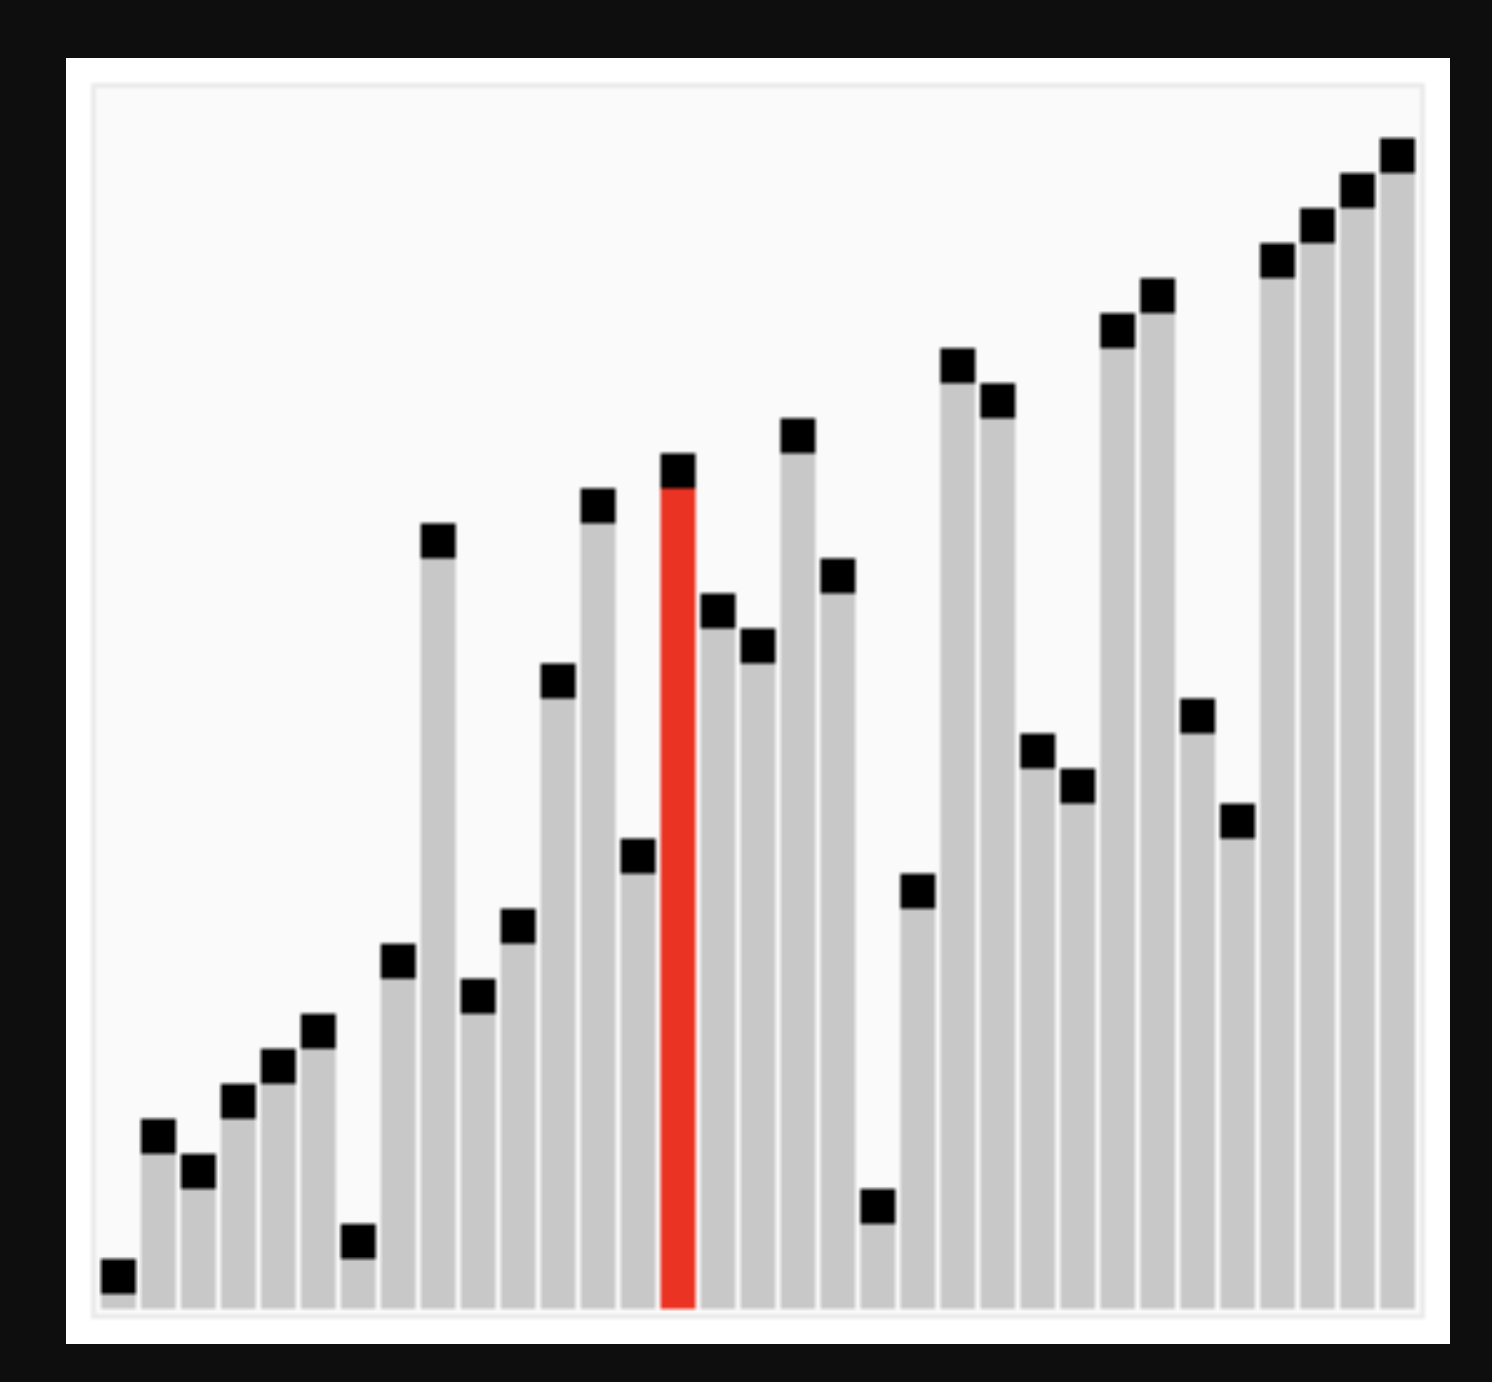
\includegraphics[width=\textwidth]{../images/bsort_gif.png}

  (\href{https://upload.wikimedia.org/wikipedia/commons/5/54/Sorting_bubblesort_anim.gif}{animation})
\end{minipage}

\end{footnotesize}
\end{frame}

\subsection{Selection sort}
\begin{frame}[fragile]
\begin{footnotesize}

  \head{Selection sort}

  \begin{itemize}
  \item Udtræk det mindste element i listen.
  \item Gentag processen rekursivt indtil der ikke længere er elementer i listen.
  \end{itemize}

  \head{En implementation i F\#:}

\begin{lstlisting}[numbers=none,frame=none,mathescape]
let rec select (xs:int list) (m,ys) =
  match xs with
    | [] -> (m,ys)
    | x::xs -> if x < m then select xs (x,m::ys)
               else select xs (m,x::ys)

let rec ssort xs =
  match xs with
    | [] -> []
    | x::xs -> let (m,xs) = select xs (x,[])
               in m::ssort xs
\end{lstlisting}

\end{footnotesize}
\end{frame}

\begin{frame}[fragile]
\begin{footnotesize}

\head{Analyse af selection sort}

\vspace{1ex}

\begin{minipage}[b]{0.55\textwidth}

  Funktionen \lstinline{select} køres $N$ gange og for hver kørsel
  gennemløbes listen (i gennemsnit $N/2$ elementer).

\vspace{1ex}

\head{Summary:}

\vspace{1ex}
  \begin{tabular}{ll}
    Best time: & $O(N^2)$ \\
    Worst time: & $O(N^2)$ \\
    Average time: & $O(N^2)$
  \end{tabular}

  \vfill
\mbox{ }
\end{minipage} \hspace{1cm}
\begin{minipage}[b]{0.3\textwidth}

  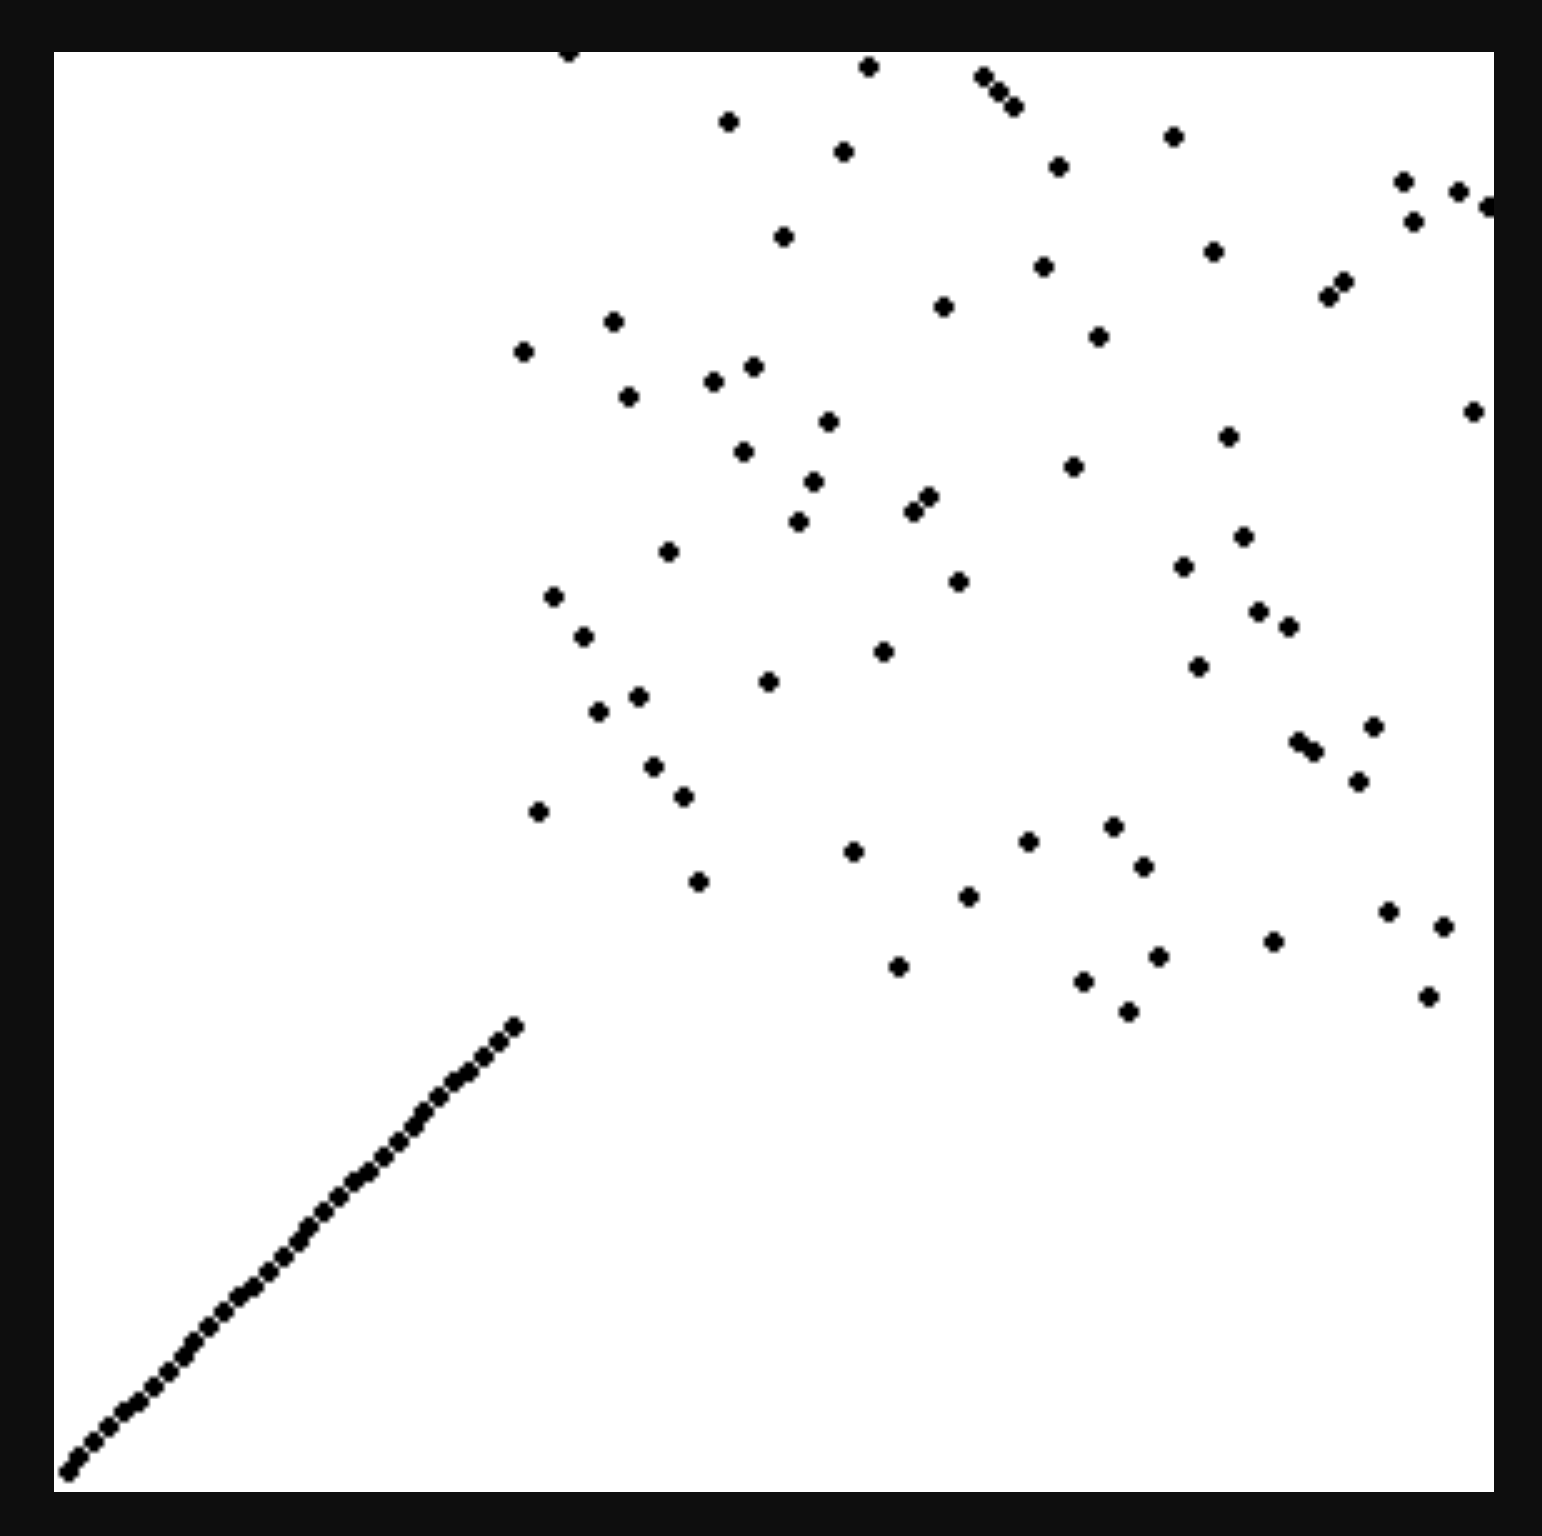
\includegraphics[width=\textwidth]{../images/ssort_gif.png}

  (\href{https://upload.wikimedia.org/wikipedia/commons/b/b0/Selection_sort_animation.gif}{animation})
\end{minipage}

\end{footnotesize}
\end{frame}

\subsection{Mergesort}
\begin{frame}[fragile]
\begin{footnotesize}

  \head{Mergesort --- divide-and-conquer (del-og-hersk!)}

  \emph{John von Neumann, 1945}

  \begin{itemize}
  \item Opdel listen i to lige store dele.
  \item Sort\'er (rekursivt) hver liste.
  \item Flet (merge) de to resultater.
  \end{itemize}

  \head{En implementation i F\#:}

\begin{lstlisting}[numbers=none,frame=none,mathescape]
let rec msort xs =
  let sz = List.length xs
  if sz < 2 then xs
  else let n = sz / 2
       let ys = xs.[0..n-1]
       let zs = xs.[n..sz-1]
       in merge (msort ys) (msort zs)
\end{lstlisting}

\head{Bemærk:}
\begin{itemize}
\item Mergesort benytter sig af slice-syntaksen (e.g., \lstinline{xs.[0..n-1]}) for at udtrække dele af en liste.
\item Mergesort benytter sig af utility-funktionen \lstinline{merge} (next slide).
\end{itemize}
\end{footnotesize}
\end{frame}

\begin{frame}[fragile]
\begin{footnotesize}
\head{Utility-funktionen \lstinline{merge}}

\vspace{1ex}

\begin{lstlisting}[numbers=none,frame=none,mathescape]
let rec merge xs ys =
  match xs, ys with
    | [], _ -> ys
    | _, [] -> xs
    | x::xs, y::ys -> if x<y then x::merge xs (y::ys)
                      else y::merge (x::xs) ys
\end{lstlisting}

\head{Bemærk:}
\begin{itemize}
\item Funktionen \lstinline{merge} fletter to sorterede lister sammen således at resultatet er sorteret.
\end{itemize}

\end{footnotesize}
\end{frame}

\begin{frame}[fragile]
\begin{footnotesize}
\head{Analyse af Mergesort}

\vspace{1ex}

\begin{minipage}[b]{0.55\textwidth}

  Kald-træet for \lstinline{msort} er $\log(N)$ dybt og
  \lstinline{merge} kaldes i hver knude. Det viser sig at Best time =
  Worst time = Average time = $O(N\log(N))$.

\vspace{1ex}

\head{Summary:}

\vspace{1ex}
  \begin{tabular}{ll}
    Best time: & $O(N\log(N))$ \\
    Worst time: & $O(N\log(N))$ \\
    Average time: & $O(N\log(N))$
  \end{tabular}

  \vfill
\mbox{ }
\end{minipage} \hspace{1cm}
\begin{minipage}[b]{0.3\textwidth}

  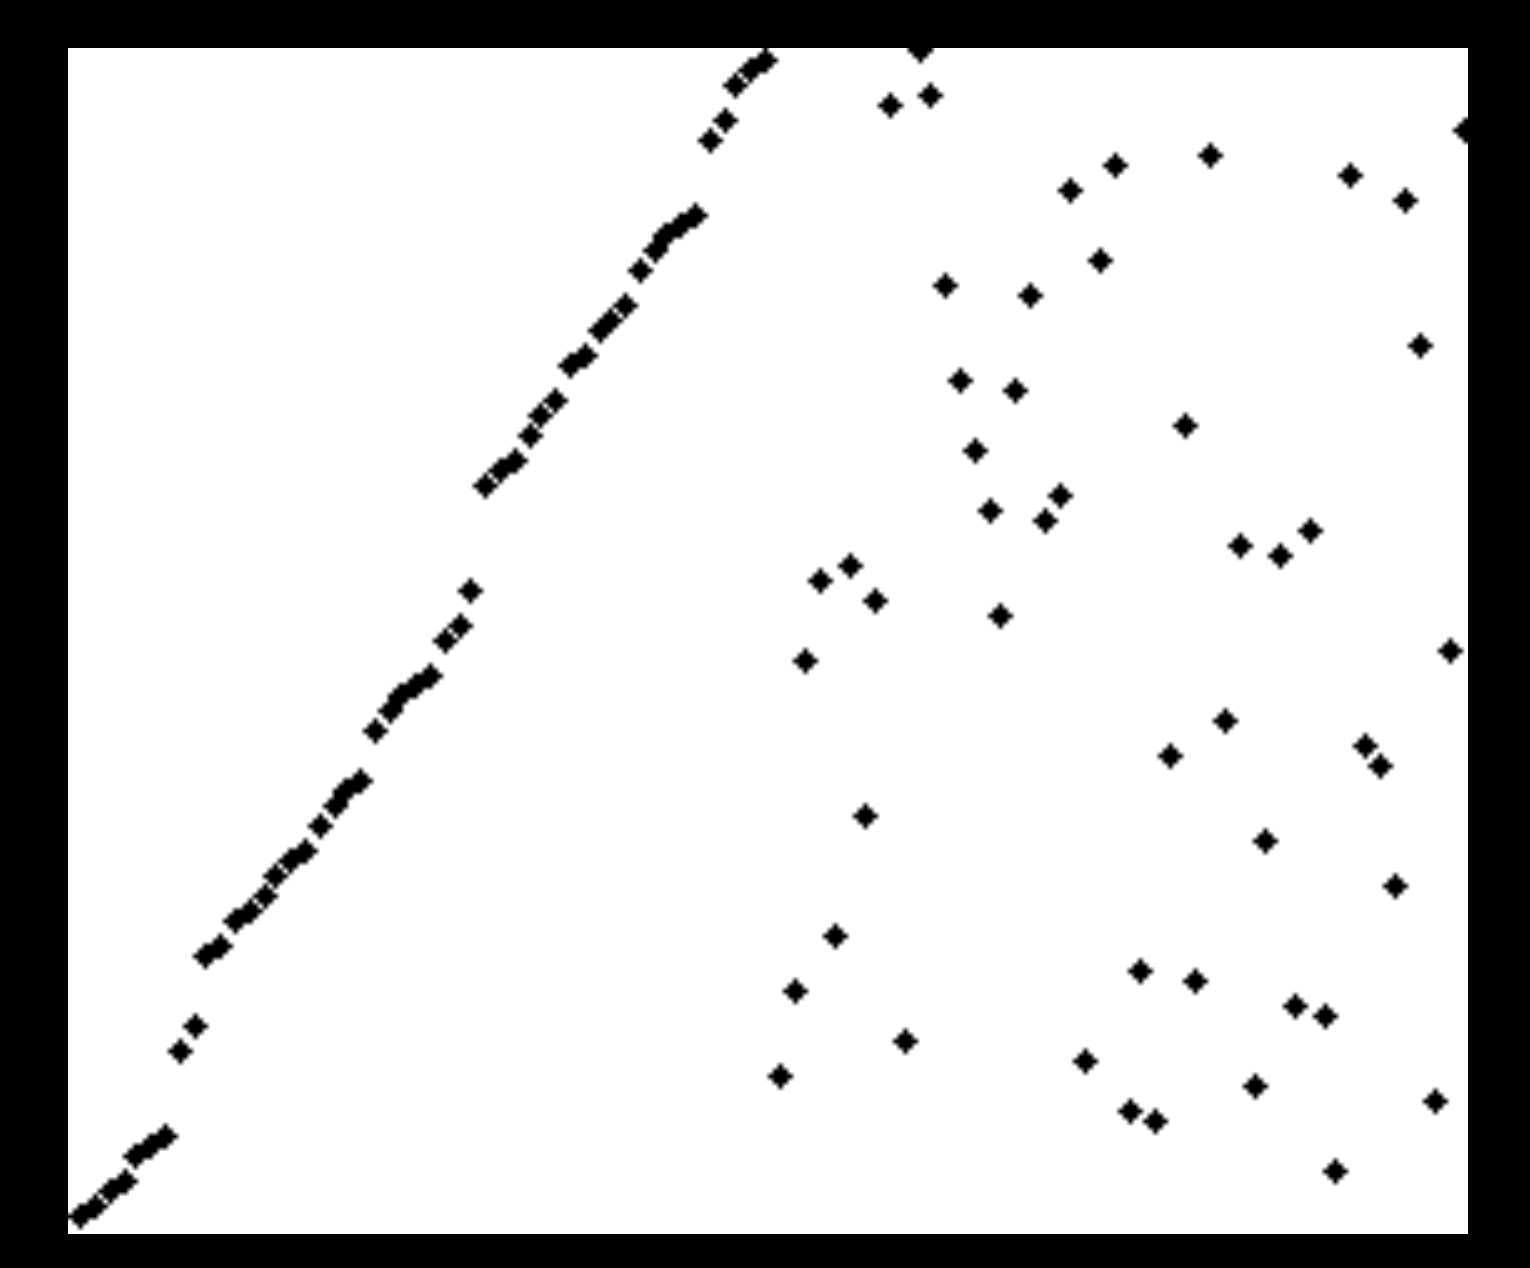
\includegraphics[width=\textwidth]{../images/msort_gif.png}

  (\href{https://upload.wikimedia.org/wikipedia/commons/c/c5/Merge_sort_animation2.gif}{animation})
\end{minipage}

\end{footnotesize}
\end{frame}

\subsection{Quicksort}
\begin{frame}[fragile]
\begin{footnotesize}

  \head{Quicksort --- divide-and-conquer (del-og-hersk!)}

  \emph{Tony Hoare, 1959}

  \begin{itemize}
  \item Vælg et element $x$ i listen (pivot).
  \item Del listen i tre dele, dem mindre en $x$, dem lig med $x$ og dem større end $x$.
  \item Sort\'er de to lister indeholdende henholdsvis små og store elementer.
  \item Sammensæt de tre lister.
  \end{itemize}

  \head{En implementation i F\#:}

\begin{lstlisting}[numbers=none,frame=none,mathescape]
let rec qsort xs =
  if List.isEmpty xs then xs
  else let pivot = xs.[0]
       let (xs, es, ys) = partition pivot xs
       in qsort xs @ es @ qsort ys
\end{lstlisting}

\head{Bemærk:}
\begin{itemize}
\item Vi vælger det første element i listen som pivot; en bedre løsning er at vælge et tilfældigt element.
\item Quicksort benytter sig af utility-funktionen \lstinline{partition} (next slide).
\end{itemize}
\end{footnotesize}
\end{frame}

\begin{frame}[fragile]
\begin{footnotesize}
\head{Utility-funktionen \lstinline{partition}}

\vspace{1ex}

\begin{lstlisting}[numbers=none,frame=none,mathescape]
let partition y xs =
  List.foldBack (fun x (xs,es,ys) ->
                   if x < y then (x::xs,es,ys)
                   else if x > y then (xs,es,x::ys)
                   else (xs,x::es,ys)) xs ([],[],[])
\end{lstlisting}

\head{Bemærk:}
\begin{itemize}
\item Funktionen \lstinline{partition} partitionerer listen (ved brug
  af \lstinline{List.foldBack}) i de elementer der er henholdsvis mindre end
  \lstinline{y}, lig med \lstinline{y} og større end \lstinline{y}.
\end{itemize}

\end{footnotesize}
\end{frame}

\begin{frame}[fragile]
\begin{footnotesize}
\head{Analyse af Quicksort}

  Kald-træet for \lstinline{qsort} er $\log(N)$ dybt (average) og
  \lstinline{partition} kaldes i hver knude. Det viser sig at Worst time = $O(N^2)$ $>$
  Average time $O(N\log(N))$ $>$ Best time = $O(N)$.

\vspace{1ex}

\begin{minipage}[b]{0.55\textwidth}

\head{Summary:}

\vspace{1ex}
  \begin{tabular}{lll}
    Best time: & $O(N)$ & \emph{I hvilket tilfælde?} \\
    Worst time: & $O(N^2)$ & \emph{I hvilket tilfælde?} \\
    Average time: & $O(N\log(N))$
  \end{tabular}

  \vspace{1ex}
  \begin{itemize}
  \item Ved at vælge et ``random'' pivot kan risikoen for worst-time opførsel minimeres.
  \item Quicksort kan (relativt) let implementeres for arrays med in-place opdateringer og meget lidt ekstra pladsforbrug.
  \item Ved brug af forskellige ``tweaks'' kan quicksort optimeres til
    at køre ca. tre gange hurtigere end konkurenterne mergesort og
    heapsort (ikke vist her).
  \end{itemize}
  \vfill
\mbox{ }
\end{minipage} \hspace{1cm}
\begin{minipage}[b]{0.3\textwidth}

  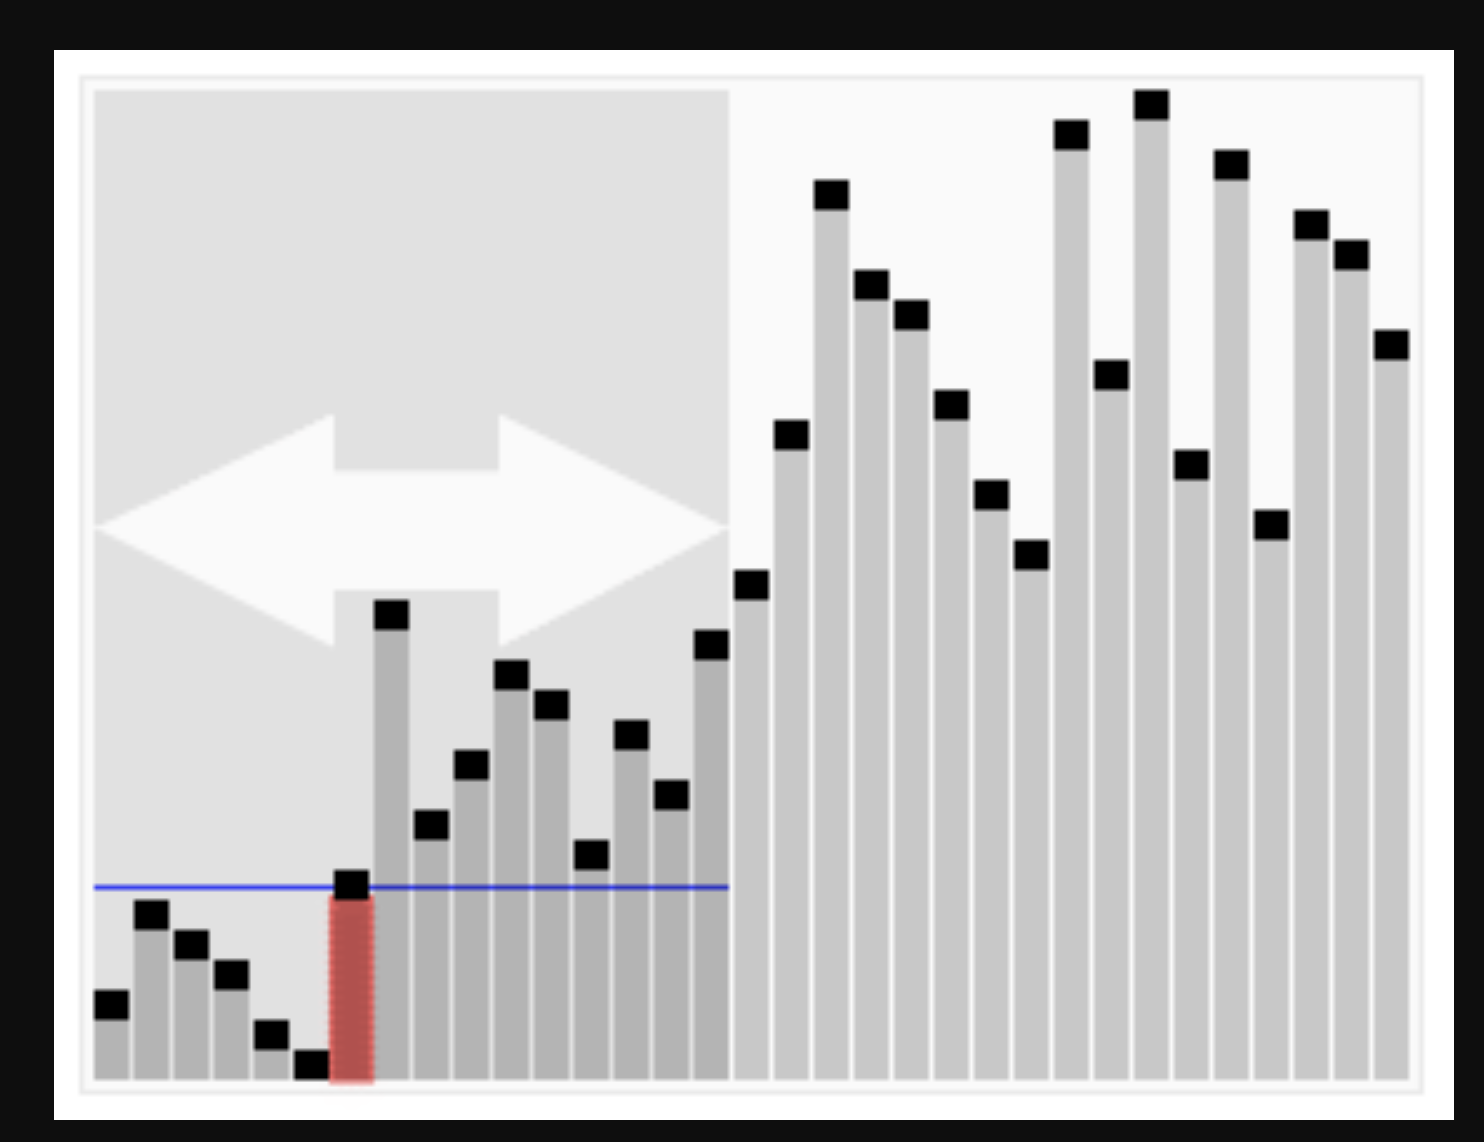
\includegraphics[width=\textwidth]{../images/qsort_gif.png}

  (\href{https://upload.wikimedia.org/wikipedia/commons/6/6a/Sorting_quicksort_anim.gif}{animation})
\end{minipage}

\end{footnotesize}
\end{frame}

\subsection*{Konklusion}
\begin{frame}[fragile]
  \headsp{Konklusion}

  \vspace{3mm}
  \tableofcontents
\end{frame}

\end{document}
